\section{Amazon Cloudfront}
\label{sec:Amazon Cloudfront}

CloudFront is a web service that speeds up distribution of your static and dynamic web content, for example, .html, .css, .php, and image files, to end users. CloudFront delivers your content through a worldwide network of data centers called edge locations. When a user requests content that you're serving with CloudFront, the user is routed to the edge location that provides the lowest latency (time delay), so content is delivered with the best possible performance. If the content is already in the edge location with the lowest latency, CloudFront delivers it immediately. If the content is not currently in that edge location, CloudFront retrieves it from an Amazon S3 bucket or an HTTP server (for example, a web server) that you have identified as the source for the definitive version of your content.
This dramatically reduces the number of networks that your users' requests must pass through, which improves performance. Users get lower latency—the time it takes to load the first byte of the object—and higher data transfer rates. You also get increased reliability and availability because copies of your objects are now held in multiple edge locations around the world.




After some initial setup, CloudFront works invisibly to speed up delivery of your content. This overview includes both the steps you perform before your first user accesses your application or website and how CloudFront serves your content when configuration is complete.
Setting up CloudFront involves a few simple steps:
How You Configure CloudFront to Deliver Your Content
You configure your origin servers, from which CloudFront gets your files for distribution from CloudFront edge locations all over the world.
An origin server stores the original, definitive version of your objects. If you're serving content over HTTP, your origin server is either an Amazon S3 bucket or an HTTP server, such as a web server. Your HTTP server can be running on an Amazon Elastic Compute Cloud (Amazon EC2) instance or on a server that you manage; these servers are also known as custom origins.
If you're distributing media files on demand using the Adobe Media Server RTMP protocol, your origin server is always an Amazon S3 bucket.
You upload your files to your origin servers. Your files, also known as objects, typically include web pages, images, and media files, but can be anything that can be served over HTTP or a supported version of Adobe RTMP, the protocol used by Adobe Flash Media Server.
If you're using an Amazon S3 bucket as an origin server, you can make the objects in your bucket publicly readable, so anyone who knows the CloudFront URLs for your objects can access them. You also have the option of keeping objects private and controlling who accesses them.
You create a CloudFront distribution, which tells CloudFront which origin servers to get your files from when users request the files through your web site or application. At the same time, you specify details such as whether you want CloudFront to log all requests and whether you want the distribution to be enabled as soon as it's created.
CloudFront sends your distribution's configuration (but not your content) to all of its edge locations—collections of servers in geographically dispersed data centers where CloudFront caches copies of your objects.
As you develop your website or application, you use the domain name that CloudFront provides for your URLs. For example, if CloudFront returns d111111abcdef8.cloudfront.net as the domain name for your distribution, the URL for logo.jpg in your Amazon S3 bucket (or in the root directory on an HTTP server) will behttp://d111111abcdef8.cloudfront.net/logo.jpg.
You can also configure your CloudFront distribution so you can use your own domain name. In that case, the URL might be http://www.example.com/logo.jpg.
Optionally, you can configure your origin server to add headers to the files; the headers indicate how long you want the files to stay in the cache in CloudFront edge locations. By default, each object stays in an edge location for 24 hours before it expires. The minimum expiration time is 0 seconds; there isn't a maximum expiration time limit. For more information, see Specifying How Long Objects Stay in a CloudFront Edge Cache (Expiration).


\begin{figure}[htb] %  figure placement: here, top, bottom
 \centering
 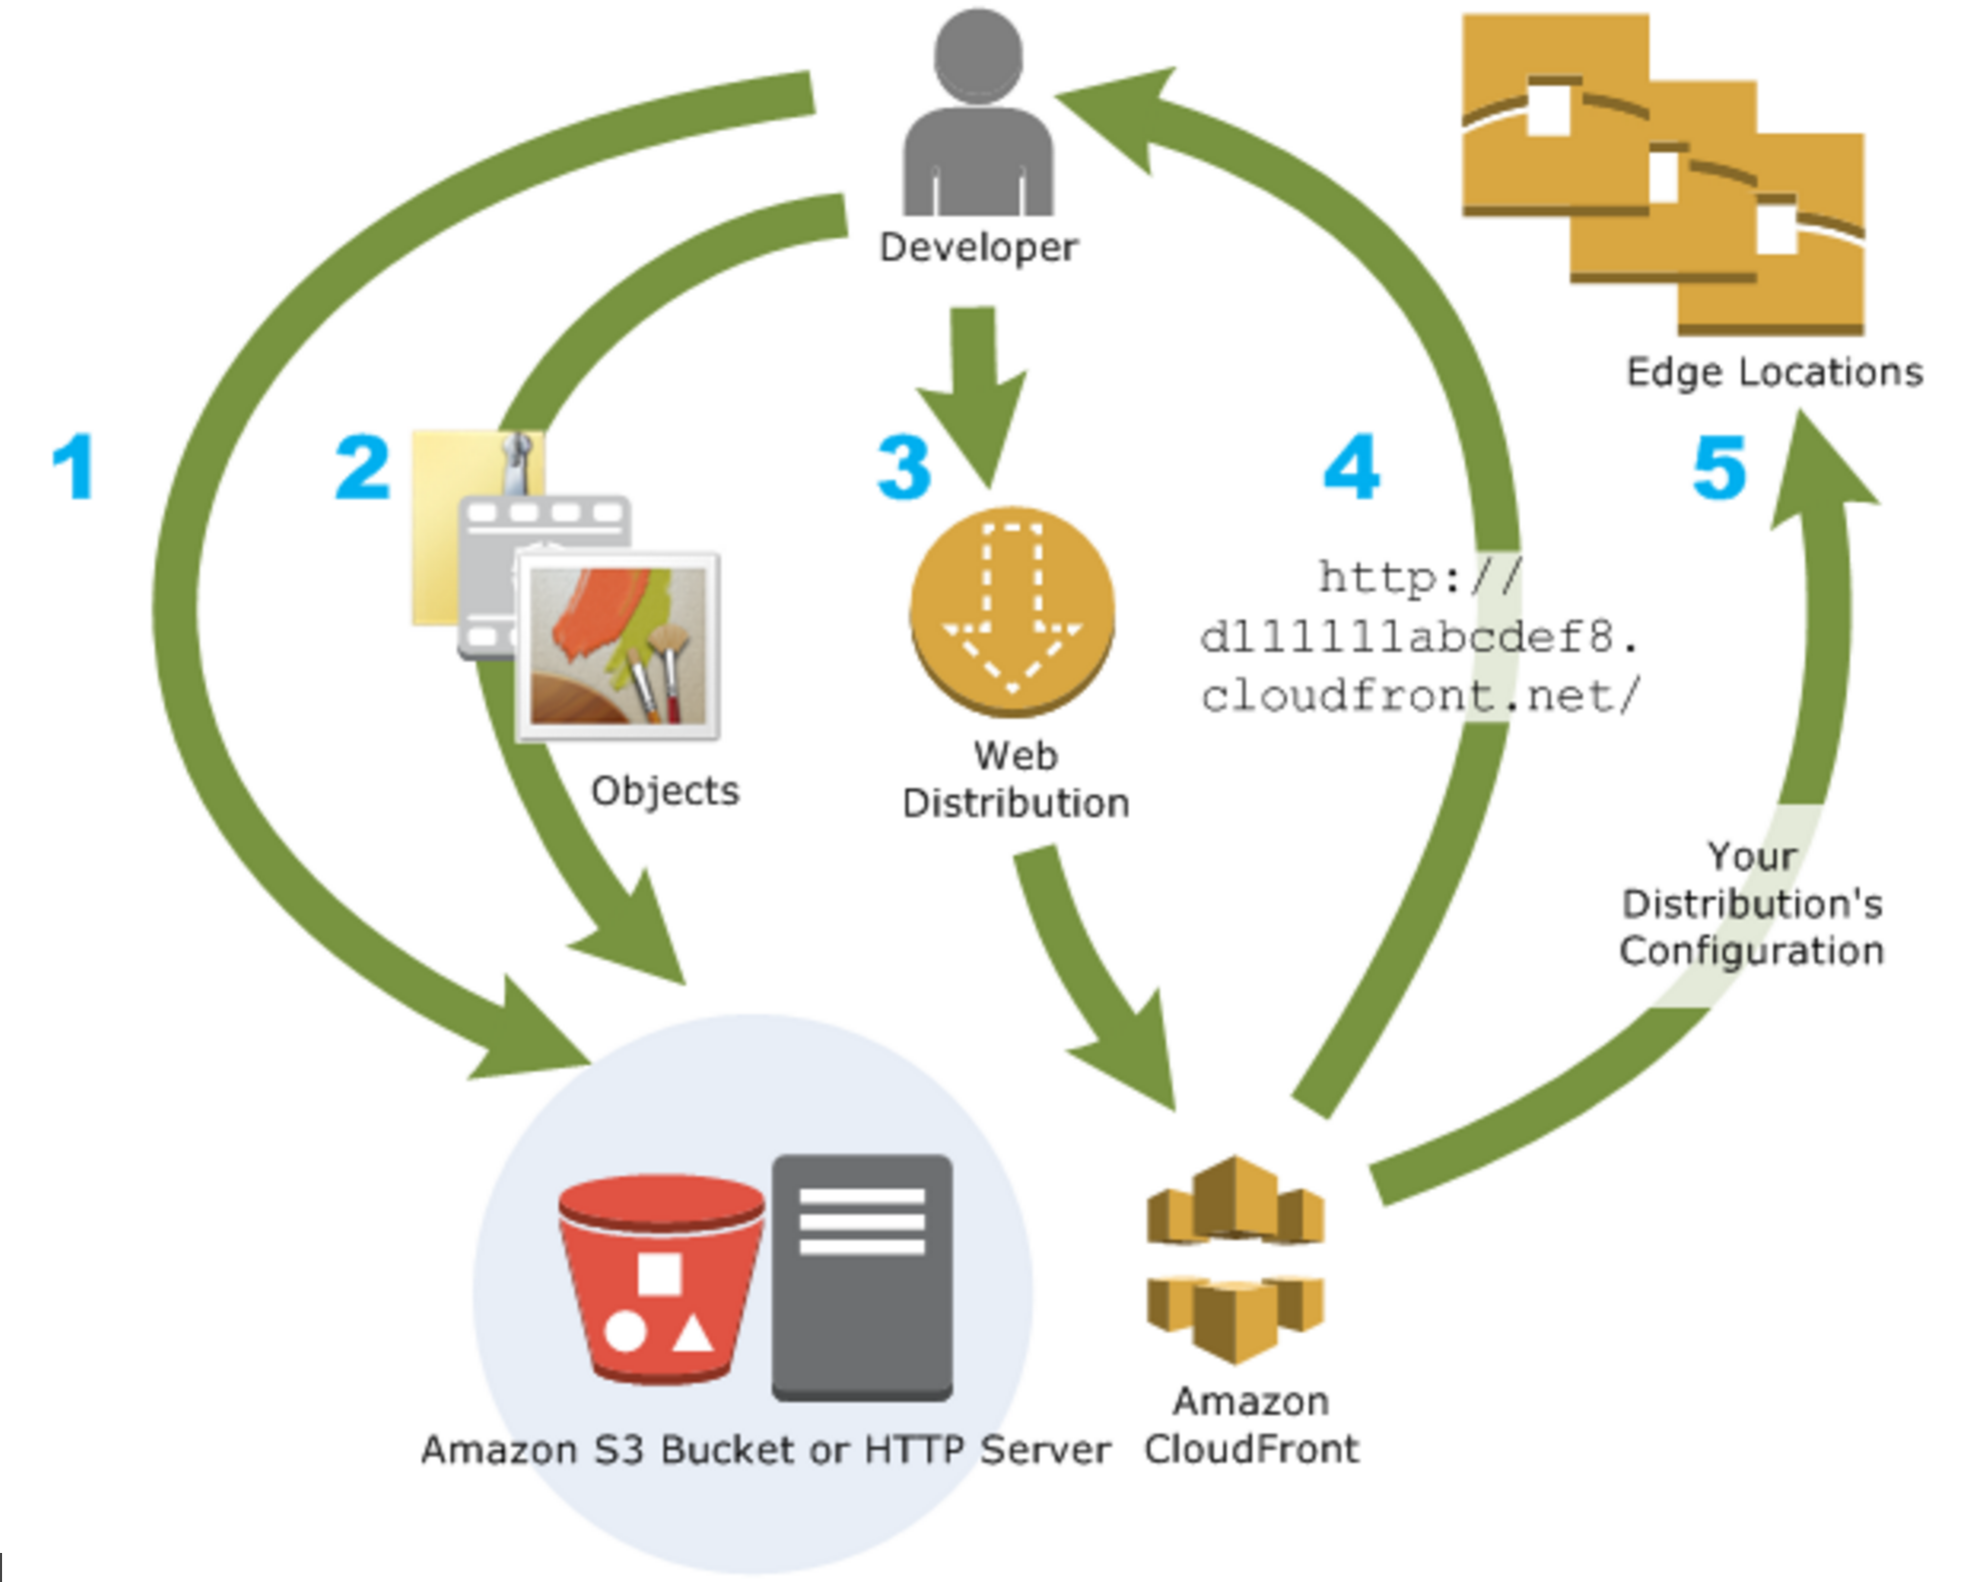
\includegraphics[width=1.0\linewidth]{images/chapter4/cloudfront.png}\hfill
 \caption[The CloudFront Lifecycle]{The CloudFront Lifecycle}
 \label{fig:fourV}
\end{figure}



How CloudFront Delivers Content to Your Users
Once you configure CloudFront to deliver your content, here's what happens when users request your objects:
A user accesses your website or application and requests one or more objects, such as an image file and an HTML file.
DNS routes the request to the CloudFront edge location that can best serve the user's request, typically the nearest CloudFront edge location in terms of latency, and routes the request to that edge location.
In the edge location, CloudFront checks its cache for the requested files. If the files are in the cache, CloudFront returns them to the user. If the files are not in the cache, it does the following:
CloudFront compares the request with the specifications in your distribution and forwards the request for the files to the applicable origin server for the corresponding file type—for example, to your Amazon S3 bucket for image files and to your HTTP server for the HTML files.
The origin servers send the files back to the CloudFront edge location.
As soon as the first byte arrives from the origin, CloudFront begins to forward the files to the user. CloudFront also adds the files to the cache in the edge location for the next time someone requests those files.
After an object has been in an edge cache for 24 hours or for the duration specified in your file headers, CloudFront does the following:
CloudFront forwards the next request for the object to your origin to determine whether the edge location has the latest version.
If the version in the edge location is the latest, CloudFront delivers it to your user.
If the version in the edge location is not the latest, your origin sends the latest version to CloudFront, and CloudFront delivers the object to your user and stores the latest version in the cache at that edge location.